% !TeX root = ../main.tex
% 离散卷积来源：materials/chapter2.pdf，第 1--8 页。

\section{本章例题集}
\label{sec:convolution-worked-examples}

\begingroup
\raggedbottom

\begin{workedexample}[有限序列卷积：列表叠加与逐点求积]
  \label{ex:lti-response-from-impulse-response}
  已知某离散时间 LTI 系统的单位脉冲响应为
  \[
    h[n]=\impulse[n+1]+\impulse[n]+2\impulse[n-1]-\impulse[n-2],
  \]
  输入为
  \[
    x[n]=3\impulse[n+1]+2\impulse[n]+\impulse[n-1]-\impulse[n-2].
  \]
  求输出 $y[n]$。先用线性、时不变性列表叠加，再用卷积和的翻转平移法逐个计算 $n=-2,-1,\ldots,4$ 的样值。已知序列见\cref{fig:ex-lti-superposition-given}。

  \begin{figure}[H]
    \centering
    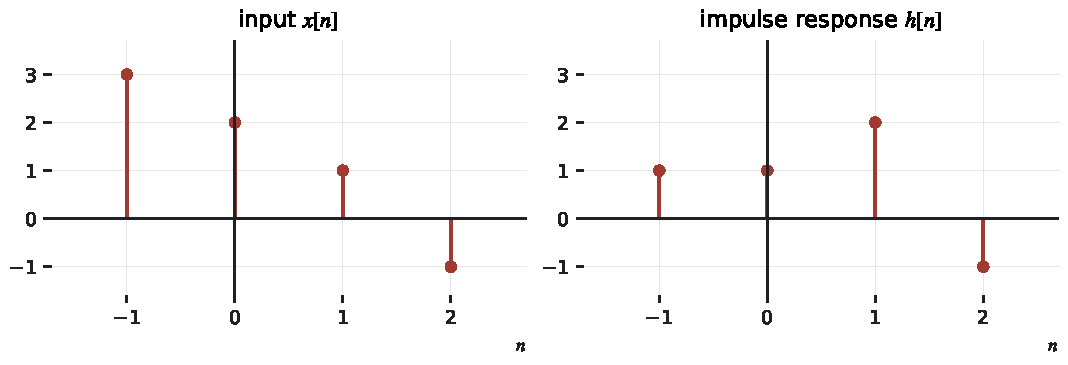
\includegraphics[width=0.86\textwidth]{04-convolution/examples/lti-superposition-given.pdf}
    \caption{例题 \ref{ex:lti-response-from-impulse-response} 的输入 $x[n]$ 与单位脉冲响应 $h[n]$。}
    \label{fig:ex-lti-superposition-given}
  \end{figure}
\end{workedexample}

\begin{solution}
  \textbf{方法一：列表叠加。}

  由 $\impulse[n]\longrightarrow h[n]$ 以及线性、时不变性，输入的四个脉冲分量分别产生
  \[
    3h[n+1],\qquad 2h[n],\qquad h[n-1],\qquad -h[n-2].
  \]
  因此
  \[
    y[n]=3h[n+1]+2h[n]+h[n-1]-h[n-2].
  \]

  $x[n]$ 与 $h[n]$ 的首尾下标均为 $-1,2$，所以输出的计算范围为 $-2\le n\le4$，共 $4+4-1=7$ 个位置。按输出下标对齐各分量：
  \[
  \begin{array}{c|rrrrrrr}
    n&-2&-1&0&1&2&3&4\\ \hline
    3h[n+1]&3&3&6&-3&0&0&0\\
    2h[n]&0&2&2&4&-2&0&0\\
    h[n-1]&0&0&1&1&2&-1&0\\
    -h[n-2]&0&0&0&-1&-1&-2&1\\ \hline
    y[n]&3&5&9&1&-1&-3&1
  \end{array}
  \]
  \textbf{方法二：翻转、平移，逐点求积。}

  固定 $x[k]$，先把 $h[k]$ 翻转。样值及其下标为
  \[
    \begin{array}{c|rrrr}
      k&-1&0&1&2\\ \hline
      h[k]&1&1&2&-1
    \end{array}
    \qquad\longrightarrow\qquad
    \begin{array}{c|rrrr}
      k&-2&-1&0&1\\ \hline
      h[-k]&-1&2&1&1
    \end{array}
  \]
  再把 $h[-k]$ 平移 $n$ 格，得到 $h[n-k]$。它的四个样值 $-1,2,1,1$ 依次位于 $k=n-2,n-1,n,n+1$，每次令 $n$ 增加 $1$，整行向右移一格。\Cref{fig:ex-lti-sliding-entering} 标出了 $n=-2,-1,0,1$ 时的配对关系。

  \begin{figure}[H]
    \centering
    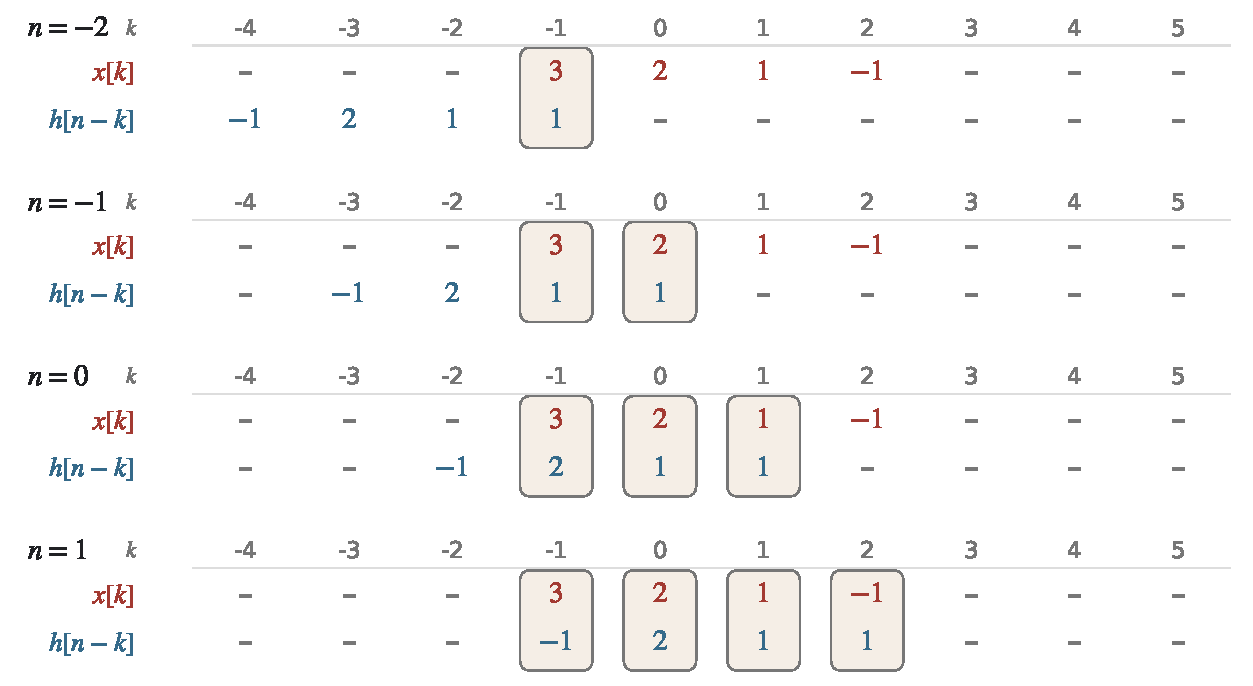
\includegraphics[width=0.96\textwidth]{04-convolution/examples/lti-sliding-entering.pdf}
    \caption{例题 \ref{ex:lti-response-from-impulse-response} 在 $n=-2,-1,0,1$ 时的逐次对齐。每框上下两数相乘，再把各框的乘积相加；短横线表示该处样值为零。}
    \label{fig:ex-lti-sliding-entering}
  \end{figure}

  从第一次接触算到完全重叠，依次得到
  \begin{align*}
    y[-2]&=3\times1=3,\\
    y[-1]&=3\times1+2\times1=3+2=5,\\
    y[0]&=3\times2+2\times1+1\times1=6+2+1=9,\\
    y[1]&=3\times(-1)+2\times2+1\times1+(-1)\times1\\
         &=-3+4+1-1=1.
  \end{align*}
  例如 $n=0$ 时，参与求和的横坐标为 $k=-1,0,1$，所以第三行的配对具体是
  \[
    y[0]=x[-1]h[1]+x[0]h[0]+x[1]h[-1].
  \]
  这里两个因子的下标每对都相加为 $0$。一般计算 $y[n]$ 时，每对下标都应相加为 $n$，可用来检查配对。

  继续向右平移，重叠点逐渐减少，见\cref{fig:ex-lti-sliding-leaving}：

  \begin{figure}[H]
    \centering
    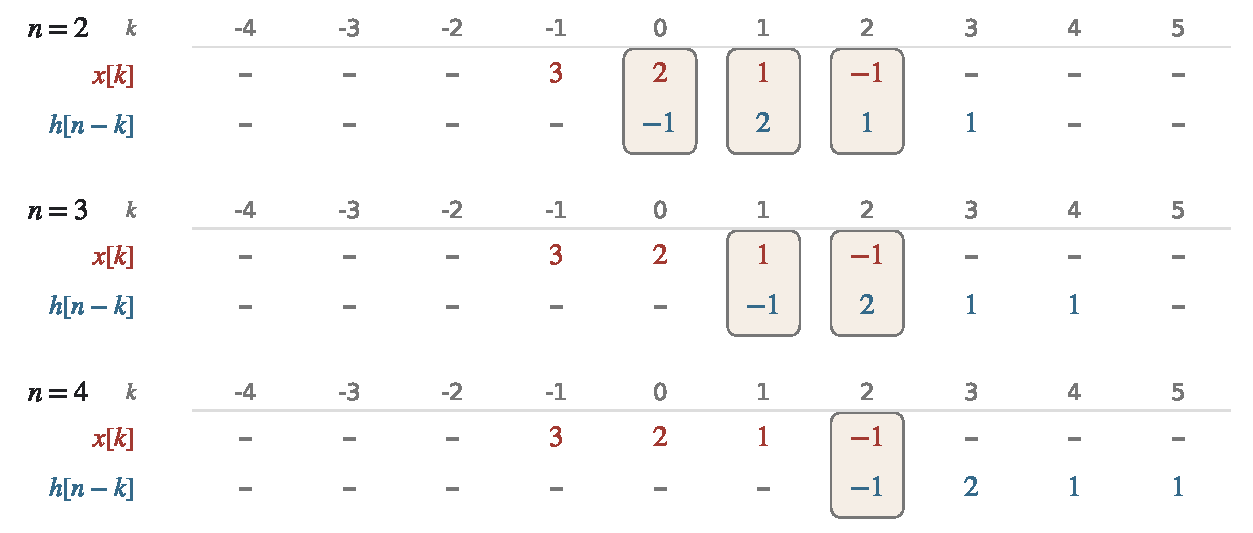
\includegraphics[width=0.96\textwidth]{04-convolution/examples/lti-sliding-leaving.pdf}
    \caption{例题 \ref{ex:lti-response-from-impulse-response} 在 $n=2,3,4$ 时的逐次对齐。保持 $x[k]$ 不动，每次把 $h[n-k]$ 向右移一格。}
    \label{fig:ex-lti-sliding-leaving}
  \end{figure}

  \begin{align*}
    y[2]&=2\times(-1)+1\times2+(-1)\times1=-2+2-1=-1,\\
    y[3]&=1\times(-1)+(-1)\times2=-1-2=-3,\\
    y[4]&=(-1)\times(-1)=1.
  \end{align*}
  当 $n<-2$ 或 $n>4$ 时，两序列没有重叠，$y[n]=0$。两种方法得到相同样值，输出可写成
  \[
    y[n]=3\impulse[n+2]+5\impulse[n+1]+9\impulse[n]
    +\impulse[n-1]-\impulse[n-2]-3\impulse[n-3]+\impulse[n-4].
  \]
  输出波形见\cref{fig:ex-lti-superposition-answer}。

  \begin{figure}[H]
    \centering
    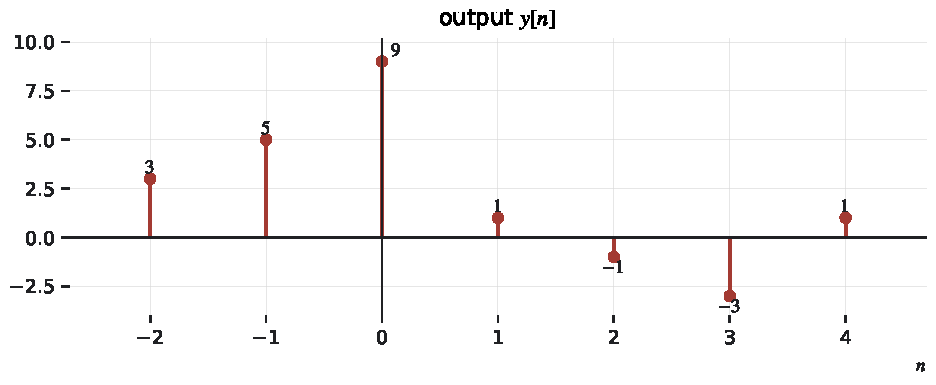
\includegraphics[width=0.72\textwidth]{04-convolution/examples/lti-superposition-answer.pdf}
    \caption{例题 \ref{ex:lti-response-from-impulse-response} 的输出。首尾下标分别为 $-2$ 与 $4$，与支撑区间检查一致。}
    \label{fig:ex-lti-superposition-answer}
  \end{figure}
\end{solution}

\begin{technique}
  先用首尾下标相加确定 $n$ 的范围。列表法把各行缩放移位的响应按\red{相同输出下标对齐}；公式法固定 $x[k]$，翻转 $h[k]$ 后每次右移一格，逐个写出当前重叠点的乘积及其和。负样值用括号保留符号，检查每对因子的下标之和是否等于当前 $n$。
\end{technique}

% 来源：materials/chapter2.pdf，第 4--5 页；补全每个 n 的求积过程。
\begin{workedexample}[含内部零样值的有限序列卷积]
  \label{ex:discrete-convolution-interior-zeros}
  设
  \[
    \begin{aligned}
      x[n]&=\impulse[n+1]+2\impulse[n]+\impulse[n-1]+\impulse[n-2],\\
      h[n]&=\impulse[n]-\impulse[n-1]-\impulse[n-4]+\impulse[n-5].
    \end{aligned}
  \]
  用列表法或翻转平移法求 $y[n]=(x\conv h)[n]$，列出每个输出下标对应的乘积与和。题设序列见\cref{fig:ex-interior-zeros-given}。

  \begin{figure}[H]
    \centering
    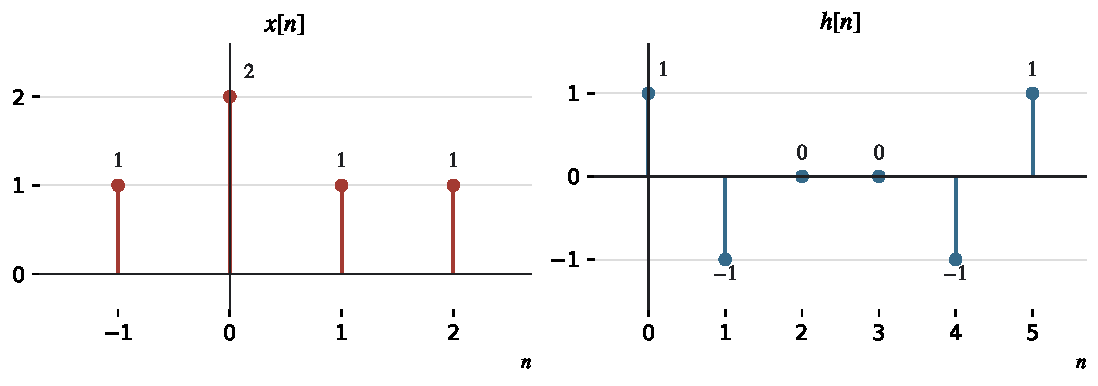
\includegraphics[width=0.86\textwidth]{04-convolution/examples/interior-zeros-given.pdf}
    \caption{例题 \ref{ex:discrete-convolution-interior-zeros} 的已知序列。$h[2]=h[3]=0$，这两个位置仍须保留。}
    \label{fig:ex-interior-zeros-given}
  \end{figure}
\end{workedexample}

\begin{solution}
  $x$ 的首尾非零下标为 $-1,2$，$h$ 的首尾非零下标为 $0,5$，所以
  \[
    n_{\min}=-1+0=-1,\qquad n_{\max}=2+5=7.
  \]
  输出共有 $4+6-1=9$ 个位置。$h$ 从下标 $0$ 到 $5$ 的完整样值为 $1,-1,0,0,-1,1$。先按输出下标列出移位响应并相加：
  \[
    \begin{array}{c|rrrrrrrrr}
      n&-1&0&1&2&3&4&5&6&7\\ \hline
      h[n+1]&1&-1&0&0&-1&1&0&0&0\\
      2h[n]&0&2&-2&0&0&-2&2&0&0\\
      h[n-1]&0&0&1&-1&0&0&-1&1&0\\
      h[n-2]&0&0&0&1&-1&0&0&-1&1\\ \hline
      y[n]&1&1&-1&0&-2&-1&1&0&1
    \end{array}
  \]

  用翻转平移法复算时，先写出翻转后的样值：
  \[
    \begin{array}{c|rrrrrr}
      k&-5&-4&-3&-2&-1&0\\ \hline
      h[-k]&1&-1&0&0&-1&1
    \end{array}
  \]
  翻转后零值仍各占一个位置，平移时整行移动。

  逐个列出同一下标处的乘积，按 $k$ 从小到大求和：
  \[
    \begin{array}{c|c|l}
      n&\text{共同区间内的 }k&\text{乘积之和 }y[n]\\ \hline
      -1&-1&1\times1=1\\
      0&-1,0&1\times(-1)+2\times1=1\\
      1&-1,0,1&1\times0+2\times(-1)+1\times1=-1\\
      2&-1,0,1,2&1\times0+2\times0+1\times(-1)+1\times1=0\\
      3&-1,0,1,2&1\times(-1)+2\times0+1\times0+1\times(-1)=-2\\
      4&-1,0,1,2&1\times1+2\times(-1)+1\times0+1\times0=-1\\
      5&0,1,2&2\times1+1\times(-1)+1\times0=1\\
      6&1,2&1\times1+1\times(-1)=0\\
      7&2&1\times1=1
    \end{array}
  \]
  例如 $n=2$ 时，四项分别是 $x[-1]h[3]$、$x[0]h[2]$、$x[1]h[1]$、$x[2]h[0]$。前两项因 $h[3]=h[2]=0$ 消失，后两项为 $-1$ 与 $1$，相加也为零。因此，$y[2]=0$ 是\red{乘积相消}的结果。$y[6]=0$ 同样来自 $1-1$。

  范围外没有重叠，输出为零；范围内样值及波形见\cref{fig:ex-interior-zeros-answer}。

  \begin{figure}[H]
    \centering
    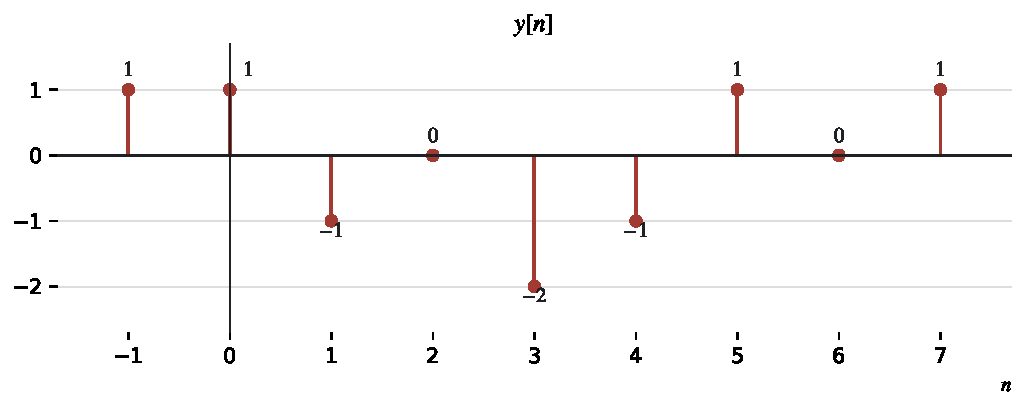
\includegraphics[width=0.76\textwidth]{04-convolution/examples/interior-zeros-answer.pdf}
    \caption{例题 \ref{ex:discrete-convolution-interior-zeros} 的输出。$n=2,6$ 处的零值仍属于首尾下标之间的九个位置。}
    \label{fig:ex-interior-zeros-answer}
  \end{figure}
\end{solution}

\begin{technique}
  先按整数下标写齐序列，\red{内部零值必须占位}。删掉 $h[2],h[3]$ 会把后面的 $-1,1$ 错移两格。算完每个 $n$ 的乘积再求和；有重叠时仍可能得到零输出，不能把首尾范围内的零值跳过。
\end{technique}

\begin{workedexample}[右边指数序列与单位阶跃的卷积]
  \label{ex:geometric-step-convolution}
  已知离散时间 LTI 系统的输入与单位脉冲响应分别为
  \[
    x[n]=a^n\stepfun[n],
    \qquad
    h[n]=\stepfun[n],
  \]
  其中 $a$ 为常数。用卷积和求输出 $y[n]$，并分别讨论 $a\neq1$ 与 $a=1$。\Cref{fig:ex-geometric-step-given} 以 $a=1/2$ 为例示意题设信号。

  \begin{figure}[H]
    \centering
    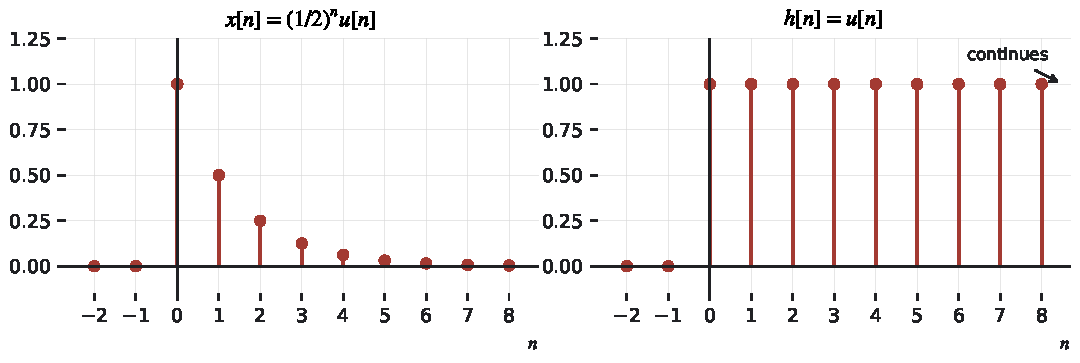
\includegraphics[width=0.86\textwidth]{04-convolution/examples/geometric-step-given.pdf}
    \caption{例题 \ref{ex:geometric-step-convolution} 的输入与单位脉冲响应示意图（取 $a=1/2$）。}
    \label{fig:ex-geometric-step-given}
  \end{figure}
\end{workedexample}

\begin{solution}
  先写出样值：$x[k]$ 从 $k=0$ 起依次为 $1,a,a^2,a^3,\ldots$，$h[k]$ 从 $k=0$ 起恒为 $1$。$h[-k]$ 翻转后在 $k\leq0$ 上为 $1$；平移后，$h[n-k]$ 在 $k\leq n$ 上为 $1$。

  当 $n<0$ 时，$x[k]$ 要求 $k\geq0$，两行没有重叠，$y[n]=0$。从 $n=0$ 开始逐次右移，前四个样值的计算为
  \begin{align*}
    y[0]&=1\times1=1,\\
    y[1]&=1\times1+a\times1=1+a,\\
    y[2]&=1\times1+a\times1+a^2\times1=1+a+a^2,\\
    y[3]&=1\times1+a\times1+a^2\times1+a^3\times1=1+a+a^2+a^3.
  \end{align*}
  每右移一格，原有乘积保留，并新增 $x[n]\times1=a^n$。\Cref{fig:ex-geometric-step-sliding} 给出了前四次对齐。

  \begin{figure}[H]
    \centering
    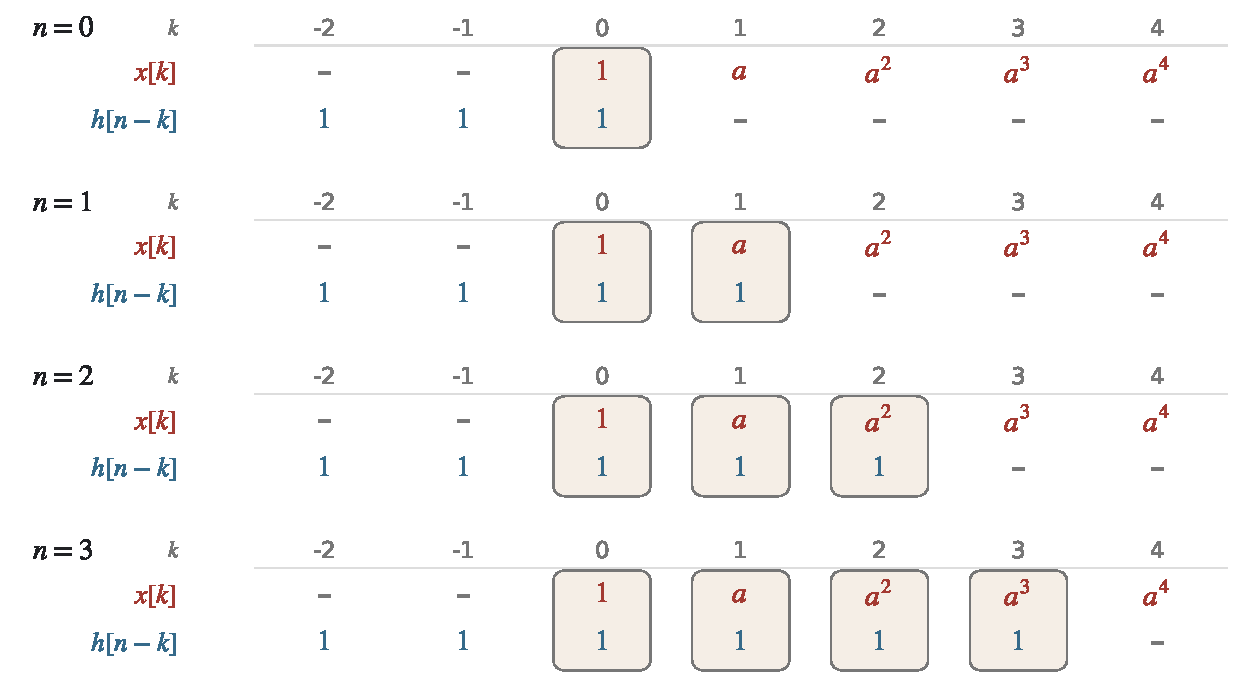
\includegraphics[width=0.94\textwidth]{04-convolution/examples/geometric-step-sliding.pdf}
    \caption{例题 \ref{ex:geometric-step-convolution} 在 $n=0,1,2,3$ 时的翻转平移。每次向右移动一格，新增一个参与求和的样值。}
    \label{fig:ex-geometric-step-sliding}
  \end{figure}

  对一般的 $n\geq0$，卷积和为
  \[
    y[n]
    =\sum_{k=-\infty}^{\infty}a^k\stepfun[k]\stepfun[n-k].
  \]
  两个阶跃因子分别要求 $k\geq0$ 与 $k\leq n$，所以
  \[
    y[n]=1\times1+a\times1+\cdots+a^n\times1
    =1+a+\cdots+a^n=\sum_{k=0}^{n}a^k.
  \]
  这里共有 $n+1$ 项。若 $a\neq1$，有限等比数列给出
  \[
    y[n]=\frac{1-a^{n+1}}{1-a}\stepfun[n].
  \]
  若 $a=1$，则每一项都为 $1$，故
  \[
    y[n]=(n+1)\stepfun[n].
  \]
  以 $a=1/2$ 为例，输出从 $1$ 起逐渐趋近于 $2$，见\cref{fig:ex-geometric-step-answer}。

  \begin{figure}[H]
    \centering
    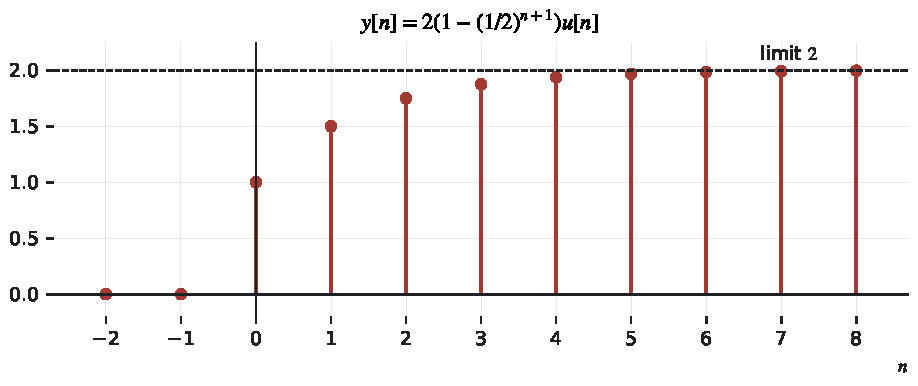
\includegraphics[width=0.72\textwidth]{04-convolution/examples/geometric-step-answer.pdf}
    \caption{例题 \ref{ex:geometric-step-convolution} 在 $a=1/2$ 时的输出；虚线为极限值 $2$。}
    \label{fig:ex-geometric-step-answer}
  \end{figure}
\end{solution}

\begin{technique}
  先算 $n=0,1,2,3$，观察每次平移新增的乘积；再由 $k\geq0$ 与 $k\leq n$ 写出一般求和范围 $0\leq k\leq n$。\red{零下标也算一项}，因此最后一项是 $a^n$，项数是 $n+1$。有限等比和只需单独处理 $a=1$，不要求 $|a|<1$。
\end{technique}

\par
\endgroup

\begin{workedexample}[两个右边指数信号的卷积]
  \label{ex:causal-exponential-convolution}
  设
  \[
    x(t)=\e^{-bt}\stepfun(t),
    \qquad
    h(t)=\e^{-at}\stepfun(t),
    \qquad a,b>0.
  \]
  求 $y(t)=x(t)\conv h(t)$，并讨论 $a=b$ 的特殊情形。\Cref{fig:ex-causal-exponential-given} 以 $a=1,b=2$ 为例示意两个信号。

  \begin{figure}[htbp]
    \centering
    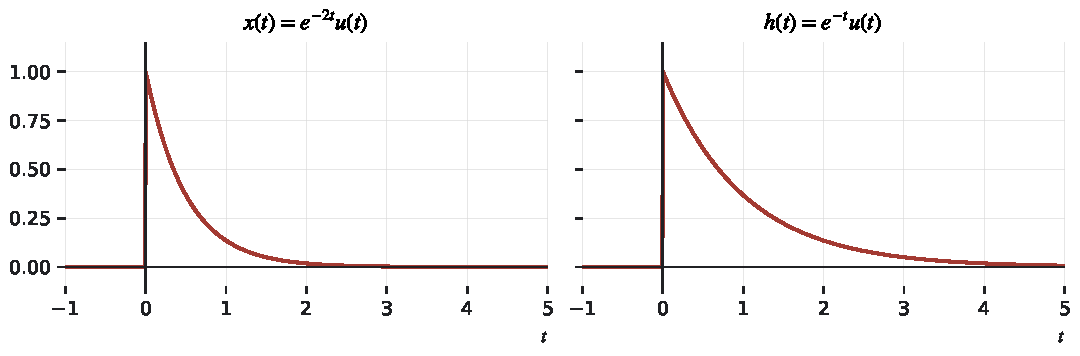
\includegraphics[width=0.82\textwidth]{04-convolution/examples/causal-exponential-given.pdf}
    \caption{例题 \ref{ex:causal-exponential-convolution} 的两个右边指数信号（取 $a=1,b=2$）。}
    \label{fig:ex-causal-exponential-given}
  \end{figure}
\end{workedexample}

\begin{solution}
  代入卷积积分：
  \[
    y(t)=\int_{-\infty}^{\infty}
    \e^{-b\tau}\stepfun(\tau)
    \e^{-a(t-\tau)}\stepfun(t-\tau)\dd\tau.
  \]
  两个阶跃分别要求 $\tau\geq0$ 与 $\tau\leq t$。当 $t<0$ 时没有重叠；当 $t\geq0$ 时，积分区间为 $0\leq\tau\leq t$。若 $a\neq b$，
  \begin{align*}
    y(t)
    &=\e^{-at}\int_0^t\e^{-(b-a)\tau}\dd\tau\\
    &=\e^{-at}\left[-\frac{\e^{-(b-a)\tau}}{b-a}\right]_0^t\\
    &=\frac{\e^{-at}}{b-a}\bigl(1-\e^{-(b-a)t}\bigr)
      =\frac{\e^{-at}-\e^{-bt}}{b-a},\qquad t\geq0.
  \end{align*}
  加上 $t<0$ 时的零值，结果为
  $y(t)=(\e^{-at}-\e^{-bt})\stepfun(t)/(b-a)$。
  若 $a=b$，被积函数中的指数因子相消，故
  \[
    y(t)=t\e^{-at}\stepfun(t).
  \]
  $a=1,b=2$ 时的输出见\cref{fig:ex-causal-exponential-answer}。

  \begin{figure}[htbp]
    \centering
    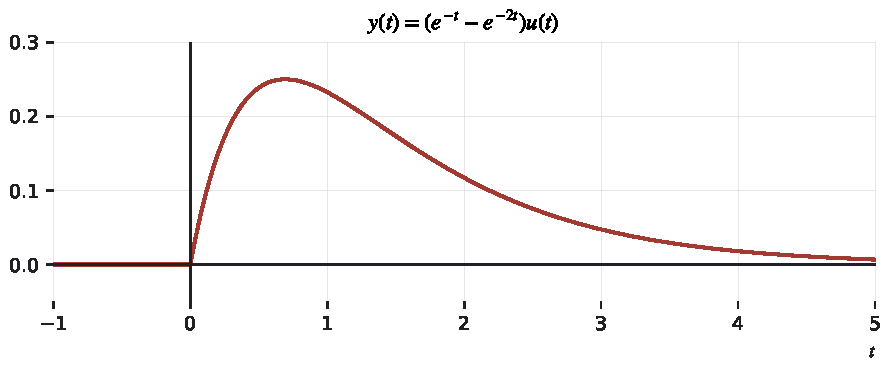
\includegraphics[width=0.68\textwidth]{04-convolution/examples/causal-exponential-answer.pdf}
    \caption{例题 \ref{ex:causal-exponential-convolution} 在 $a=1,b=2$ 时的输出。}
    \label{fig:ex-causal-exponential-answer}
  \end{figure}
\end{solution}

\begin{technique}
  连续卷积中出现阶跃时，先把每个阶跃翻译成对积分变量的限制，再取交集。本题的有效区间是 $0\leq\tau\leq t$；它既给出积分上下限，也直接说明输出是右边信号。参数恰好相等时应回到积分本身，不能把 $a=b$ 直接代入含 $b-a$ 的结果。
\end{technique}

\begin{workedexample}[矩形脉冲与有限斜坡的卷积]
  \label{ex:rectangle-ramp-convolution}
  设
  \[
    x(t)=\stepfun(t)-\stepfun(t-1),
    \qquad
    h(t)=(1-t)\bigl[\stepfun(t)-\stepfun(t-1)\bigr].
  \]
  用图解卷积思想求 $y(t)=x(t)\conv h(t)$。题设波形见\cref{fig:ex-rectangle-ramp-given}。

  \begin{figure}[htbp]
    \centering
    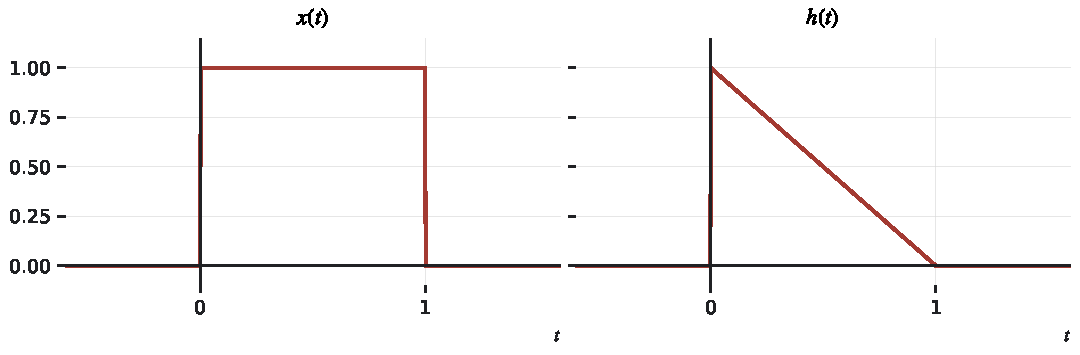
\includegraphics[width=0.82\textwidth]{04-convolution/examples/rectangle-ramp-given.pdf}
    \caption{例题 \ref{ex:rectangle-ramp-convolution} 的单位矩形与有限斜坡。}
    \label{fig:ex-rectangle-ramp-given}
  \end{figure}
\end{workedexample}

\begin{solution}
  两个信号的支撑区间均为 $[0,1]$，所以输出支撑区间为 $[0,2]$。翻转平移后
  \[
    h(t-\tau)=1-t+\tau
  \]
  在 $t-1\leq\tau\leq t$ 上非零，而 $x(\tau)$ 要求 $0\leq\tau\leq1$。

  当 $0\leq t\leq1$ 时，端点次序为 $t-1\leq0\leq t\leq1$，交集为 $[0,t]$，故
  \[
    y(t)=\int_0^t(1-t+\tau)\dd\tau
    =\left[(1-t)\tau+\frac{\tau^2}{2}\right]_0^t
    =t-\frac{t^2}{2}.
  \]
  当 $1\leq t\leq2$ 时，端点次序为 $0\leq t-1\leq1\leq t$，交集为 $[t-1,1]$，故
  \[
    y(t)=\int_{t-1}^{1}(1-t+\tau)\dd\tau
    =\left[(1-t)\tau+\frac{\tau^2}{2}\right]_{t-1}^{1}
    =\frac{(2-t)^2}{2}.
  \]
  在\cref{fig:ex-continuous-ramp-sliding} 中，阴影是相乘后的积分区域：进入时为梯形，离开时为三角形。
  \begin{figure}[H]
    \centering
    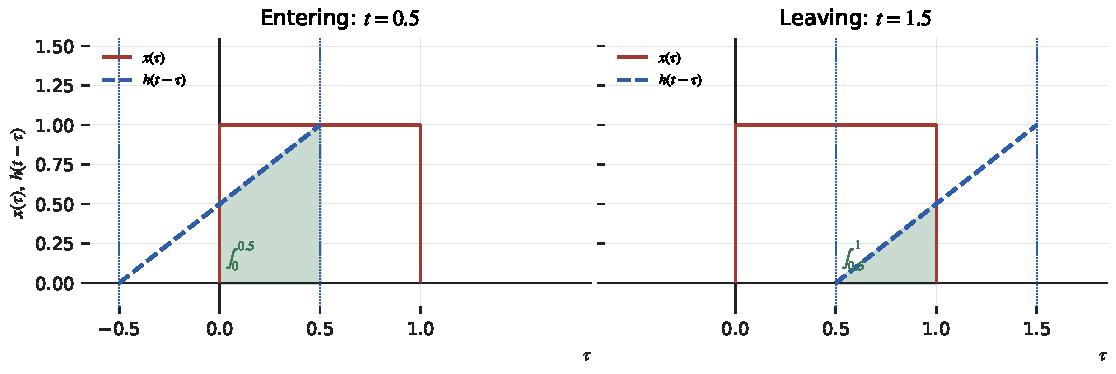
\includegraphics[width=0.88\textwidth]{04-convolution/examples/ramp-sliding.pdf}
    \caption{矩形与斜坡的两种重叠状态。横坐标为积分变量 $\tau$，$t$ 是固定的输出时刻。}
    \label{fig:ex-continuous-ramp-sliding}
  \end{figure}
  因此
  \[
    y(t)=
    \begin{cases}
      t-t^2/2, & 0\leq t\leq1,\\
      (2-t)^2/2, & 1\leq t\leq2,\\
      0, & \text{其他}.
    \end{cases}
  \]
  输出见\cref{fig:ex-rectangle-ramp-answer}，并在 $t=1$ 处连续衔接为 $1/2$。

  \begin{figure}[htbp]
    \centering
    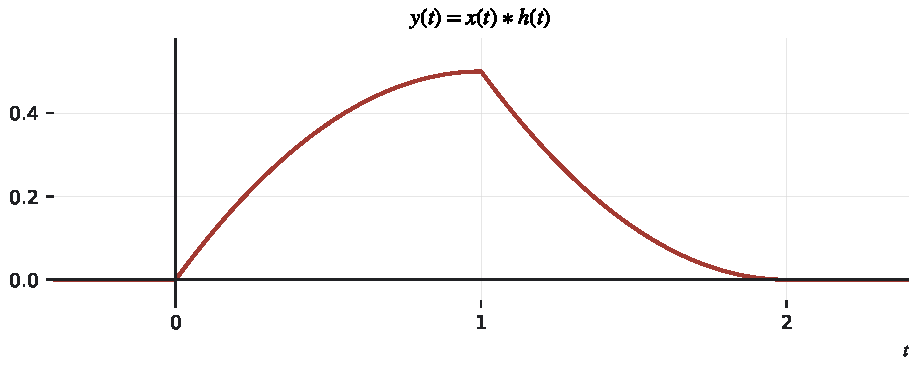
\includegraphics[width=0.68\textwidth]{04-convolution/examples/rectangle-ramp-answer.pdf}
    \caption{例题 \ref{ex:rectangle-ramp-convolution} 的分段二次输出。}
    \label{fig:ex-rectangle-ramp-answer}
  \end{figure}
\end{solution}

\begin{technique}
  图解法的分段点来自支撑端点刚好接触或越过彼此的位置。本题只需检查 $t=0,1,2$。每个区间内先写出两个支撑条件的交集，再积分；最后用分段连接处的函数值检查是否漏项或写错上下限。
\end{technique}

\begin{workedexample}[两个等宽矩形脉冲的卷积]
  \label{ex:equal-width-rectangle-convolution}
  设
  \[
    x(t)=E_1\bigl[\stepfun(t+T_0)-\stepfun(t-T_0)\bigr],
    \qquad
    h(t)=E_2\bigl[\stepfun(t+T_0)-\stepfun(t-T_0)\bigr],
  \]
  其中 $T_0>0$。求二者卷积，并说明输出的几何形状。\Cref{fig:ex-equal-width-rectangle-given} 以 $E_1=E_2=1,T_0=1$ 为例。

  \begin{figure}[htbp]
    \centering
    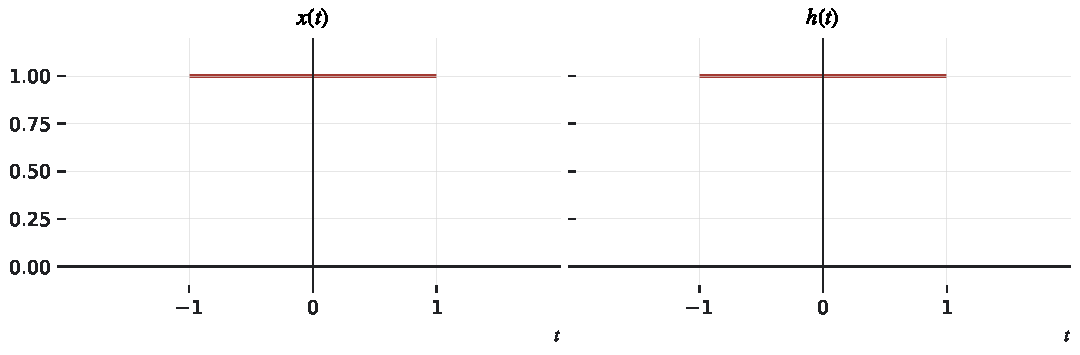
\includegraphics[width=0.82\textwidth]{04-convolution/examples/equal-rectangle-given.pdf}
    \caption{例题 \ref{ex:equal-width-rectangle-convolution} 的两个等宽矩形脉冲。}
    \label{fig:ex-equal-width-rectangle-given}
  \end{figure}
\end{workedexample}

\begin{solution}
  $h$ 关于原点对称，翻转后形状不变；平移后，$h(t-\tau)$ 的支撑是 $[t-T_0,t+T_0]$。固定的 $x(\tau)$ 支撑在 $[-T_0,T_0]$。
  在重叠区内，被积函数恒为 $E_1E_2$。从左向右滑动，分别计算：
  \begin{enumerate}
    \item $t<-2T_0$：$t+T_0<-T_0$，两个矩形尚未接触，$y(t)=0$。
    \item $-2T_0\leq t\leq0$：重叠区为 $[-T_0,t+T_0]$，
    \[
      y(t)=\int_{-T_0}^{t+T_0}E_1E_2\dd\tau
      =E_1E_2\bigl[(t+T_0)-(-T_0)\bigr]
      =E_1E_2(t+2T_0).
    \]
    \item $0\leq t\leq2T_0$：重叠区为 $[t-T_0,T_0]$，
    \[
      y(t)=\int_{t-T_0}^{T_0}E_1E_2\dd\tau
      =E_1E_2\bigl[T_0-(t-T_0)\bigr]
      =E_1E_2(2T_0-t).
    \]
    \item $t>2T_0$：$t-T_0>T_0$，两个矩形已分离，$y(t)=0$。
  \end{enumerate}
  把进入、离开两段合并，重叠长度为
  \[
    L(t)=
    \begin{cases}
      2T_0-|t|, & |t|\leq2T_0,\\
      0, & |t|>2T_0.
    \end{cases}
  \]
  因而
  \[
    y(t)=
    \begin{cases}
      E_1E_2(2T_0-|t|), & |t|\leq2T_0,\\
      0, & |t|>2T_0.
    \end{cases}
  \]
  输出是以原点为中心的三角脉冲，底边支撑为 $[-2T_0,2T_0]$，峰值为 $2T_0E_1E_2$。单位参数下的结果见\cref{fig:ex-equal-width-rectangle-answer}。

  \begin{figure}[htbp]
    \centering
    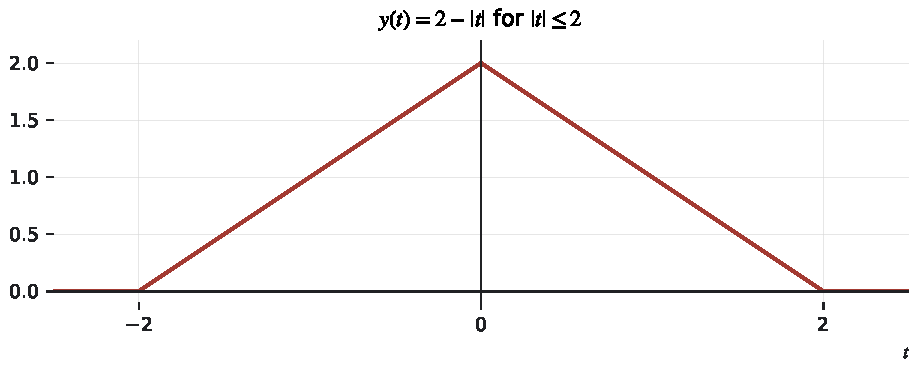
\includegraphics[width=0.68\textwidth]{04-convolution/examples/equal-rectangle-answer.pdf}
    \caption{例题 \ref{ex:equal-width-rectangle-convolution} 的三角形输出（取单位参数）。}
    \label{fig:ex-equal-width-rectangle-answer}
  \end{figure}
\end{solution}

\begin{technique}
  先画固定区间和滑动区间，再分别写出进入、离开时的积分上下限。常值矩形每段都可用“高度乘积 $\times$ 重叠长度”计算，长度等于右端减左端。等宽情形在 $t=0$ 完全重合，峰值等于脉冲宽度乘以两个高度。
\end{technique}

\begin{workedexample}[两个不等宽矩形脉冲的卷积]
  \label{ex:unequal-width-rectangle-convolution}
  设
  \[
    x(t)=E_1\bigl[\stepfun(t+a)-\stepfun(t-a)\bigr],
    \qquad
    h(t)=E_2\bigl[\stepfun(t+b)-\stepfun(t-b)\bigr],
  \]
  其中 $a\geq b>0$。求 $x(t)\conv h(t)$。\Cref{fig:ex-unequal-width-rectangle-given} 以 $a=3,b=1,E_1=E_2=1$ 为例。

  \begin{figure}[htbp]
    \centering
    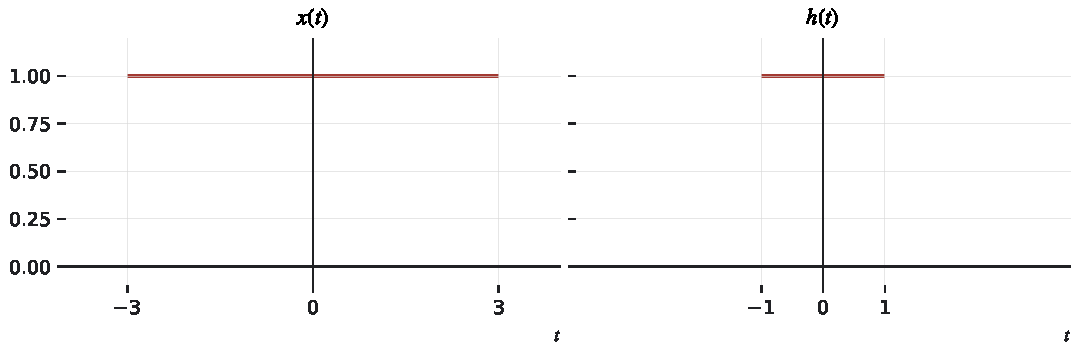
\includegraphics[width=0.82\textwidth]{04-convolution/examples/unequal-rectangle-given.pdf}
    \caption{例题 \ref{ex:unequal-width-rectangle-convolution} 的两个不等宽矩形脉冲。}
    \label{fig:ex-unequal-width-rectangle-given}
  \end{figure}
\end{workedexample}

\begin{solution}
  翻转后 $h$ 不变；$h(t-\tau)$ 的支撑区间为 $[t-b,t+b]$，固定的 $x(\tau)$ 支撑在 $[-a,a]$。四个接触时刻由滑动端点等于固定端点求得：
  \[
    t+b=-a,\quad t-b=-a,\quad t+b=a,\quad t-b=a,
  \]
  即 $t=-a-b,-a+b,a-b,a+b$。逐段计算如下：
  \[
    \begin{array}{c|c|c}
      t\text{ 的范围}&\text{重叠区间}&y(t)\\ \hline
      t<-a-b&\varnothing&0\\
      -a-b\leq t\leq-a+b&[-a,t+b]&
        E_1E_2[(t+b)-(-a)]\\
      -a+b\leq t\leq a-b&[t-b,t+b]&
        E_1E_2[(t+b)-(t-b)]\\
      a-b\leq t\leq a+b&[t-b,a]&
        E_1E_2[a-(t-b)]\\
      t>a+b&\varnothing&0
    \end{array}
  \]
  每一非零行就是在该区间上积分常数 $E_1E_2$。取 $a=3,b=1,E_1=E_2=1$，三段分别为
  \[
    \begin{aligned}
      -4\leq t\leq-2:\quad&y(t)=\int_{-3}^{t+1}1\dd\tau=t+4,\\
      -2\leq t\leq2:\quad&y(t)=\int_{t-1}^{t+1}1\dd\tau=2,\\
      2\leq t\leq4:\quad&y(t)=\int_{t-1}^{3}1\dd\tau=4-t.
    \end{aligned}
  \]
  \Cref{fig:ex-continuous-rectangle-sliding} 对照等宽和异宽矩形的进入、完全重叠与离开过程。归纳得到一般重叠长度
  \[
    L(t)=
    \begin{cases}
      2b, & |t|\leq a-b,\\
      a+b-|t|, & a-b<|t|\leq a+b,\\
      0, & |t|>a+b.
    \end{cases}
  \]
  因此
  \[
    y(t)=E_1E_2L(t).
  \]
  当较窄矩形完全落入较宽矩形时，重叠长度保持为 $2b$，因而输出中间出现平台；两侧进入和离开时，重叠长度线性变化。结果是支撑区间 $[-a-b,a+b]$、平台区间 $[-a+b,a-b]$、峰值 $2bE_1E_2$ 的梯形。示例参数下见\cref{fig:ex-unequal-width-rectangle-answer}。
  \begin{figure}[H]
    \centering
    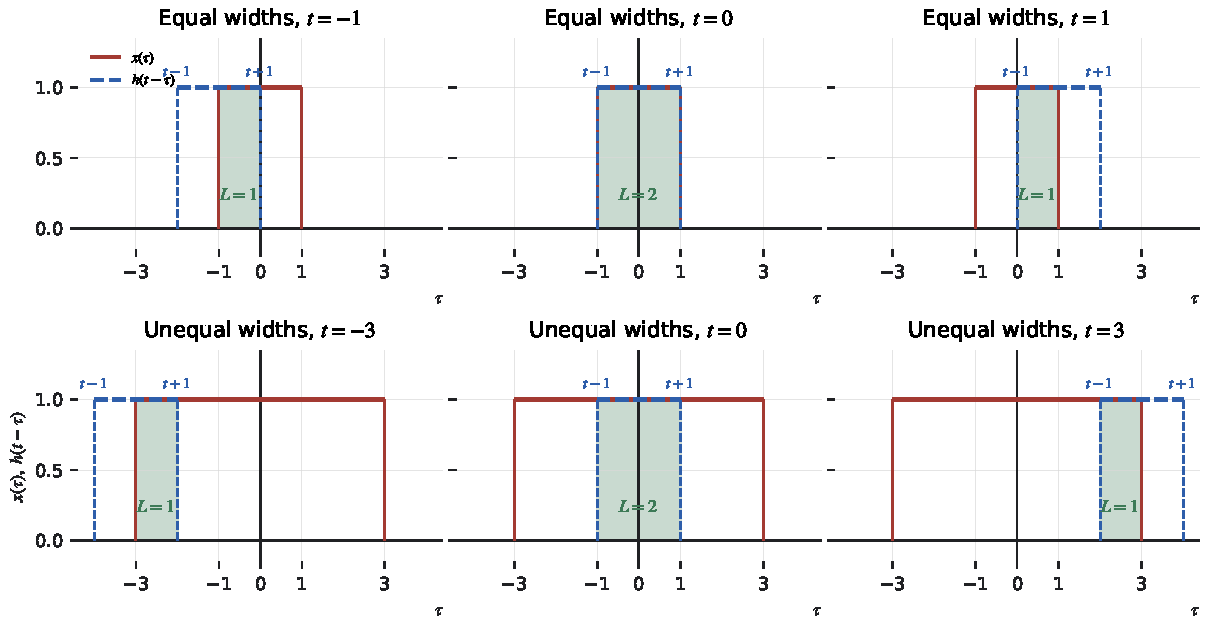
\includegraphics[width=0.94\textwidth]{04-convolution/examples/rectangle-sliding.pdf}
    \caption{等宽与异宽矩形的滑动重叠。阴影宽度决定卷积值；异宽矩形完全进入后有一段平台。}
    \label{fig:ex-continuous-rectangle-sliding}
  \end{figure}

  \begin{figure}[htbp]
    \centering
    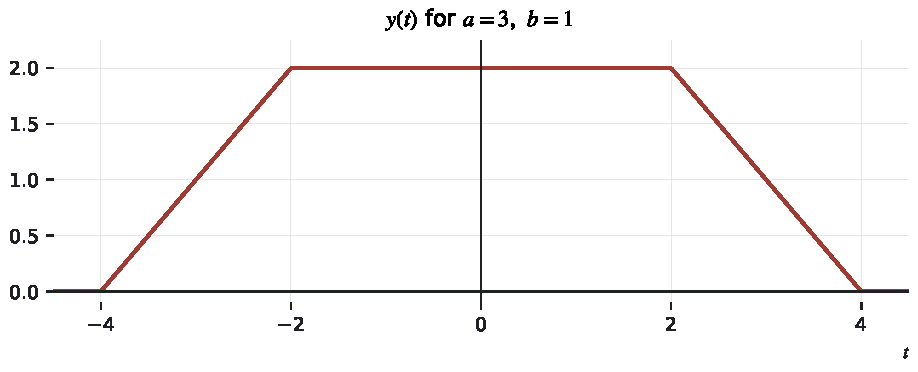
\includegraphics[width=0.68\textwidth]{04-convolution/examples/unequal-rectangle-answer.pdf}
    \caption{例题 \ref{ex:unequal-width-rectangle-convolution} 的梯形输出（取 $a=3,b=1$）。}
    \label{fig:ex-unequal-width-rectangle-answer}
  \end{figure}
\end{solution}

\begin{technique}
  对不等宽矩形，先比较半宽 $a$ 与 $b$。较窄矩形完全进入较宽矩形的范围是 $|t|\leq a-b$，对应平台；开始或结束接触发生在 $|t|=a+b$。若 $a=b$，平台宽度退化为零，梯形自然退化为三角形。
\end{technique}

\begin{workedexample}[带正负幅度的分段常值信号卷积]
  \label{ex:signed-piecewise-convolution}
  设
  \[
    x(t)=
    \begin{cases}
      1, & -1\leq t<0,\\
      -2, & 0\leq t\leq1,\\
      0, & \text{其他},
    \end{cases}
    \qquad
    h(t)=
    \begin{cases}
      1, & -1\leq t<0,\\
      2, & 0\leq t\leq1,\\
      0, & \text{其他}.
    \end{cases}
  \]
  求 $y(t)=x(t)\conv h(t)$。已知信号见\cref{fig:ex-signed-piecewise-given}。

  \begin{figure}[htbp]
    \centering
    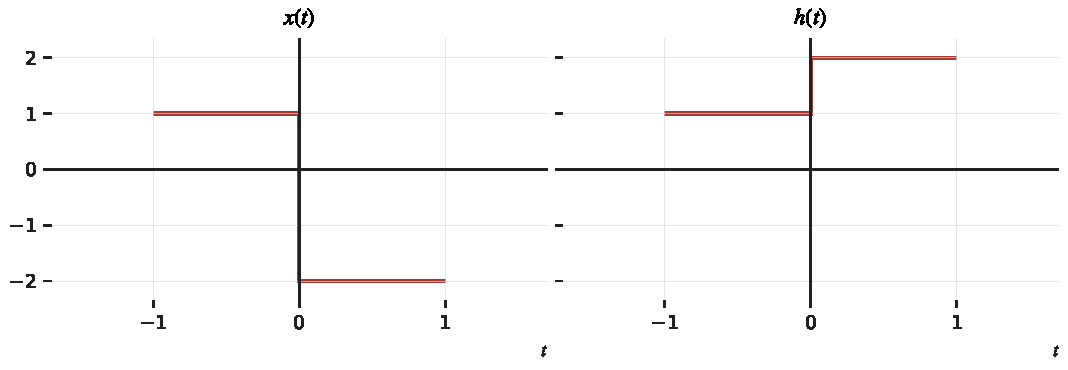
\includegraphics[width=0.82\textwidth]{04-convolution/examples/signed-piecewise-given.pdf}
    \caption{例题 \ref{ex:signed-piecewise-convolution} 的两个分段常值信号。}
    \label{fig:ex-signed-piecewise-given}
  \end{figure}
\end{workedexample}

\begin{solution}
  两个信号都支撑在 $[-1,1]$，所以输出只可能在 $[-2,2]$ 非零。先翻转 $h$：高度 $2$ 的一段移到 $[-1,0]$，高度 $1$ 的一段移到 $[0,1]$；平移后
  \[
    h(t-\tau)=
    \begin{cases}
      2,&t-1<\tau\leq t,\\
      1,&t<\tau\leq t+1,\\
      0,&\text{其他}.
    \end{cases}
  \]
  分段边界的相对次序在 $t=-2,-1,0,1,2$ 处改变。\Cref{fig:ex-continuous-signed-sliding} 给出四种重叠状态；每块都要保留两个幅度的符号。
  \begin{figure}[H]
    \centering
    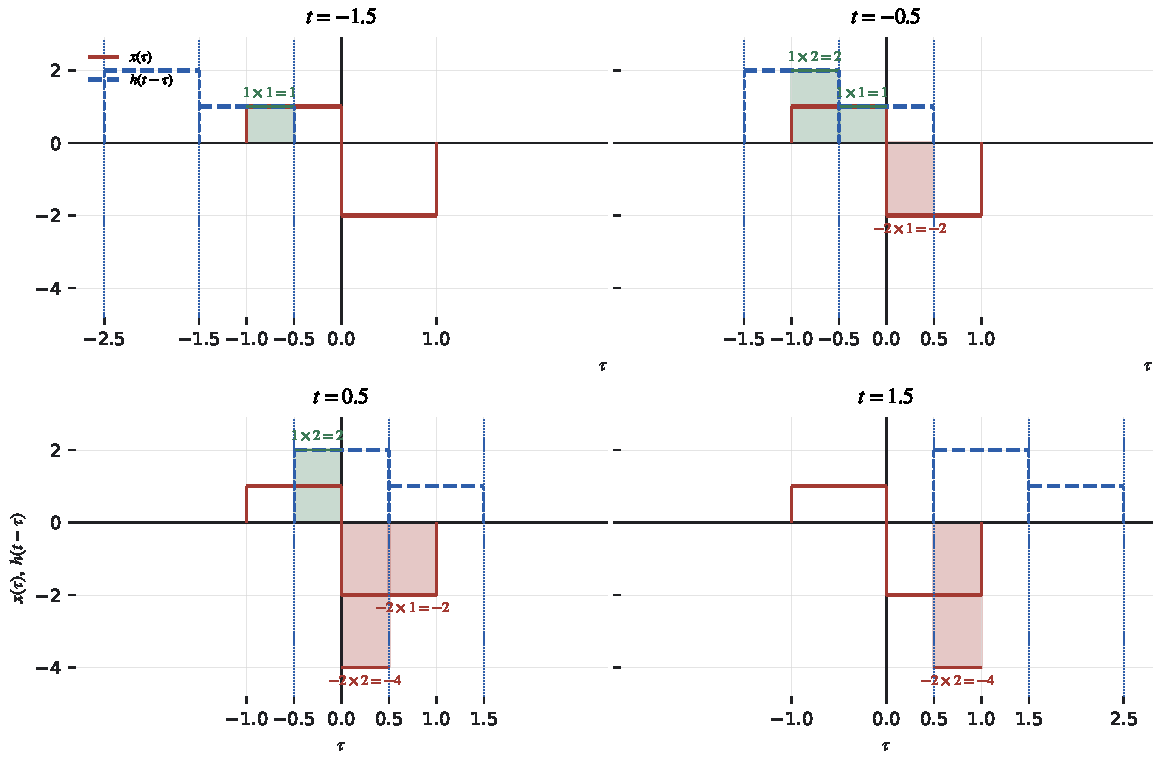
\includegraphics[width=0.88\textwidth]{04-convolution/examples/signed-sliding.pdf}
    \caption{正负分段信号的四次滑动。虚线为 $h(t-\tau)$；阴影表示乘积，横坐标为 $\tau$。}
    \label{fig:ex-continuous-signed-sliding}
  \end{figure}
  \begin{enumerate}
    \item $-2\leq t\leq-1$：只有 $[-1,t+1]$ 重叠，两个高度均为 $1$，
    \[
      y(t)=\int_{-1}^{t+1}1\cdot1\dd\tau=t+2.
    \]
    \item $-1\leq t\leq0$：沿 $\tau$ 轴分成 $[-1,t]$、$[t,0]$、$[0,t+1]$，
    \begin{align*}
      y(t)&=\int_{-1}^{t}1\cdot2\dd\tau
          +\int_t^0 1\cdot1\dd\tau
          +\int_0^{t+1}(-2)\cdot1\dd\tau\\
          &=2(t+1)+(-t)-2(t+1)=-t.
    \end{align*}
    \item $0\leq t\leq1$：分成 $[t-1,0]$、$[0,t]$、$[t,1]$，
    \begin{align*}
      y(t)&=\int_{t-1}^{0}1\cdot2\dd\tau
          +\int_0^t(-2)\cdot2\dd\tau
          +\int_t^1(-2)\cdot1\dd\tau\\
          &=2(1-t)-4t-2(1-t)=-4t.
    \end{align*}
    \item $1\leq t\leq2$：只有 $[t-1,1]$ 重叠，
    \[
      y(t)=\int_{t-1}^{1}(-2)\cdot2\dd\tau
           =-4[1-(t-1)]=4t-8.
    \]
  \end{enumerate}
  其余时刻没有重叠。汇总为
  \[
    y(t)=
    \begin{cases}
      t+2, & -2\leq t\leq-1,\\
      -t, & -1\leq t\leq0,\\
      -4t, & 0\leq t\leq1,\\
      4t-8, & 1\leq t\leq2,\\
      0, & \text{其他}.
    \end{cases}
  \]
  四段在 $t=-1,0,1$ 处分别衔接为 $1,0,-4$，与图形连续性一致；输出见\cref{fig:ex-signed-piecewise-answer}。

  \begin{figure}[htbp]
    \centering
    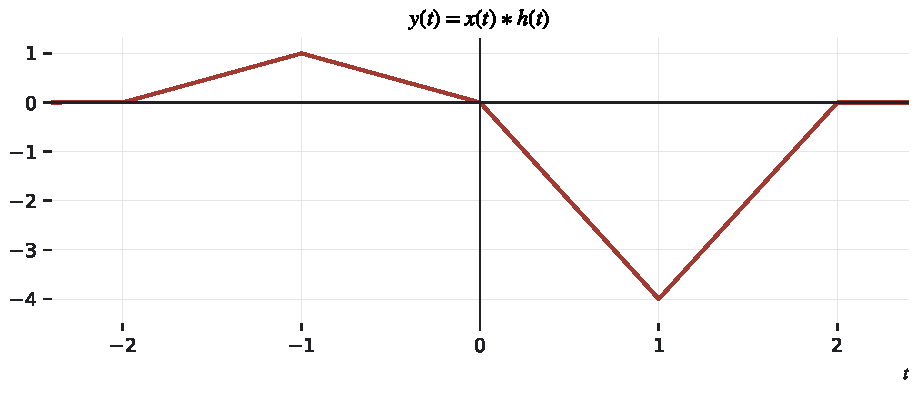
\includegraphics[width=0.68\textwidth]{04-convolution/examples/signed-piecewise-answer.pdf}
    \caption{例题 \ref{ex:signed-piecewise-convolution} 的分段线性输出。}
    \label{fig:ex-signed-piecewise-answer}
  \end{figure}
\end{solution}

\begin{technique}
  信号含正负幅度时，“重叠面积”必须理解为带符号面积。先列出所有端点相遇产生的分段时刻，再在每个区间内把重叠区域进一步按幅度切块；每块用长度乘以两个幅度，最后作代数求和。
\end{technique}

\begin{workedexample}[周期方波与三角脉冲的卷积]
  \label{ex:periodic-square-triangle-convolution}
  设 $x(t)$ 是周期为 $2$ 的方波，在一个周期内
  \[
    x(t)=
    \begin{cases}
      1, & -1\leq t<0,\\
      -1, & 0\leq t<1,
    \end{cases}
    \qquad x(t+2)=x(t),
  \]
  并令
  \[
    h(t)=
    \begin{cases}
      t, & 0\leq t\leq1,\\
      2-t, & 1<t\leq2,\\
      0, & \text{其他}.
    \end{cases}
  \]
  求 $y(t)=x(t)\conv h(t)$。题设波形见\cref{fig:ex-periodic-square-triangle-given}。

  \begin{figure}[htbp]
    \centering
    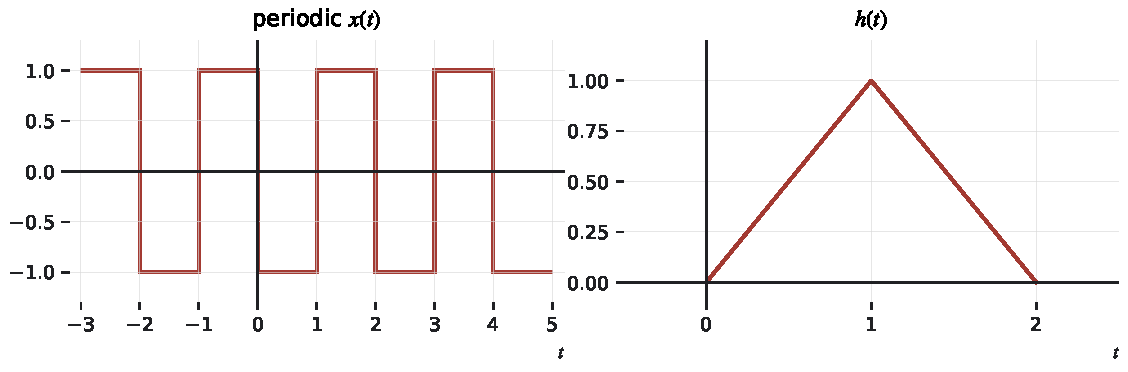
\includegraphics[width=0.86\textwidth]{04-convolution/examples/periodic-square-triangle-given.pdf}
    \caption{例题 \ref{ex:periodic-square-triangle-convolution} 的周期方波与有限三角脉冲。}
    \label{fig:ex-periodic-square-triangle-given}
  \end{figure}
\end{workedexample}

\begin{solution}
  $h$ 的支撑长度恰为 $x$ 的一个周期，输出也以 $2$ 为周期。先算完整的一个周期。翻转、平移后的三角脉冲为
  \[
    h(t-\tau)=
    \begin{cases}
      2-t+\tau,&t-2\leq\tau\leq t-1,\\
      t-\tau,&t-1<\tau\leq t,\\
      0,&\text{其他}.
    \end{cases}
  \]
  当 $0\leq t\leq1$，端点次序为 $t-2\leq-1\leq t-1\leq0\leq t$。按 $x$ 的跳变点 $-1,0$ 和三角脉冲的折点 $t-1$ 切开：
  \begin{align*}
    y(t)
    &=-\int_{t-2}^{-1}(2-t+\tau)\dd\tau
      +\int_{-1}^{t-1}(2-t+\tau)\dd\tau\\
    &\quad+\int_{t-1}^{0}(t-\tau)\dd\tau
      -\int_{0}^{t}(t-\tau)\dd\tau\\
    &=-\frac{(1-t)^2}{2}
      +\left(\frac12-\frac{(1-t)^2}{2}\right)
      +\left(\frac12-\frac{t^2}{2}\right)
      -\frac{t^2}{2}\\
    &=2t(t-1).
  \end{align*}
  当 $1\leq t\leq2$，端点次序为 $t-2\leq0\leq t-1\leq1\leq t$：
  \begin{align*}
    y(t)&=\int_{t-2}^{0}(2-t+\tau)\dd\tau
        -\int_0^{t-1}(2-t+\tau)\dd\tau\\
        &\quad-\int_{t-1}^{1}(t-\tau)\dd\tau
        +\int_1^t(t-\tau)\dd\tau\\
        &=\frac{(2-t)^2}{2}
          -\left(\frac12-\frac{(2-t)^2}{2}\right)
          -\left(\frac12-\frac{(t-1)^2}{2}\right)
          +\frac{(t-1)^2}{2}\\
        &=-2(t-1)(t-2).
  \end{align*}
  在一个周期 $0\leq t<2$ 内
  \[
    y(t)=
    \begin{cases}
      2t(t-1), & 0\leq t\leq1,\\
      -2(t-1)(t-2), & 1<t<2,
    \end{cases}
  \]
  并按周期 $2$ 延拓。由于 $x(t+1)=-x(t)$，还可用 $y(t+1)=-y(t)$ 核对第二段。输出见\cref{fig:ex-periodic-square-triangle-answer}。

  \begin{figure}[htbp]
    \centering
    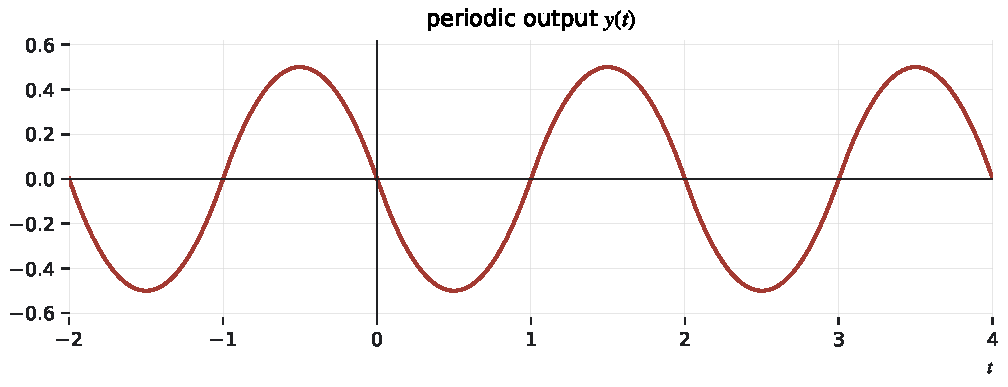
\includegraphics[width=0.78\textwidth]{04-convolution/examples/periodic-square-triangle-answer.pdf}
    \caption{例题 \ref{ex:periodic-square-triangle-convolution} 的周期输出；相邻半周期互为相反数。}
    \label{fig:ex-periodic-square-triangle-answer}
  \end{figure}
\end{solution}

\begin{technique}
  周期信号与有限长信号卷积后仍具有输入的周期。先取一个完整周期，再排列方波跳变点和滑动脉冲折点；每段都标出方波的正负号后积分。半周期反对称性可核对相邻两段，也可在熟悉切块方法后减少计算。
\end{technique}

\begin{workedexample}[由含冲激的时变换信号反求原信号]
  \label{ex:recover-signal-with-impulse}
  已知
  \[
    g(t)=x(3-2t)
    =\bigl[\stepfun(t-2)-\stepfun(t-3)\bigr]
    +2\bigl[\stepfun(t-3)-\stepfun(t-4)\bigr]
    +2\impulse(t-1).
  \]
  求 $x(t)$，并正确处理冲激在时间伸缩下的幅度。已知 $g(t)$ 见\cref{fig:ex-recover-signal-given}。

  \begin{figure}[htbp]
    \centering
    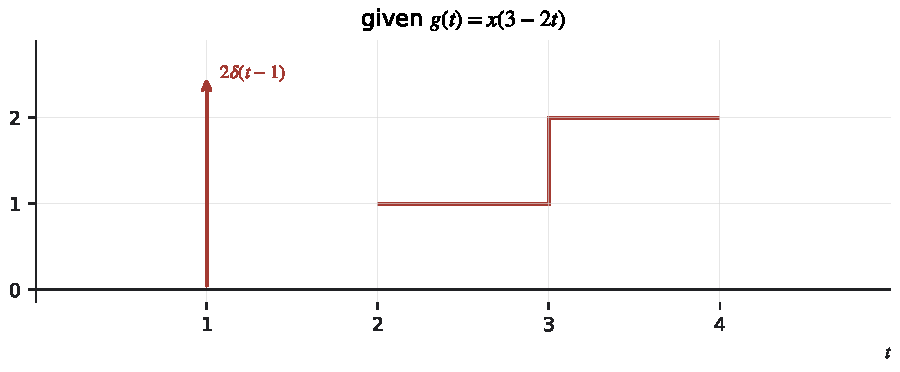
\includegraphics[width=0.72\textwidth]{04-convolution/examples/recover-signal-impulse-given.pdf}
    \caption{例题 \ref{ex:recover-signal-with-impulse} 中给定的 $g(t)=x(3-2t)$。}
    \label{fig:ex-recover-signal-given}
  \end{figure}
\end{workedexample}

\begin{solution}
  令 $s=3-2t$，则 $t=(3-s)/2$，所以
  \[
    x(s)=g\!\left(\frac{3-s}{2}\right).
  \]
  将变量名改回 $t$：
  \[
    x(t)=g\!\left(\frac{3-t}{2}\right).
  \]
  普通分段部分只需映射端点：$g$ 在 $[3,4]$ 上高度为 $2$，对应 $x$ 的区间 $[-5,-3]$；$g$ 在 $[2,3]$ 上高度为 $1$，对应区间 $[-3,-1]$。

  冲激项还会发生幅度变化：
  \begin{align*}
    2\impulse\!\left(\frac{3-t}{2}-1\right)
    &=2\impulse\!\left(-\frac12(t-1)\right)\\
    &=4\impulse(t-1).
  \end{align*}
  因此
  \[
    x(t)=2\bigl[\stepfun(t+5)-\stepfun(t+3)\bigr]
    +\bigl[\stepfun(t+3)-\stepfun(t+1)\bigr]
    +4\impulse(t-1).
  \]
  \begin{center}
    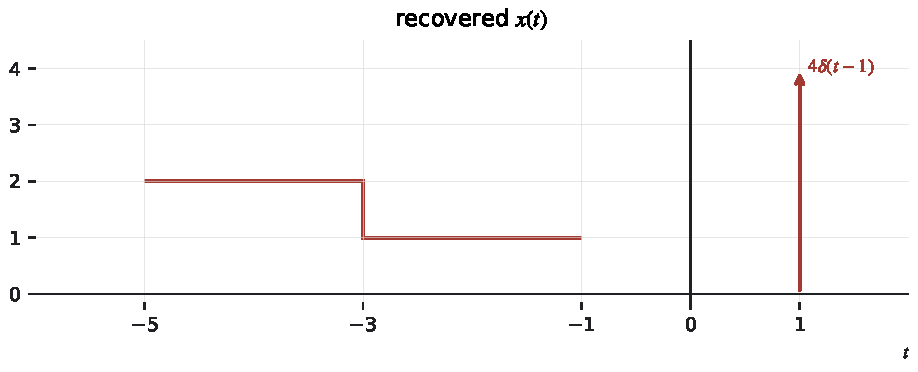
\includegraphics[width=0.38\textwidth]{04-convolution/examples/recover-signal-impulse-answer.pdf}
    \refstepcounter{figure}\label{fig:ex-recover-signal-answer}

    \small 图~\thefigure：例题 \ref{ex:recover-signal-with-impulse} 反求得到的 $x(t)$。
  \end{center}
\end{solution}

\begin{technique}
  反求复合自变量信号时，先解出原自变量再整体代回。普通函数只改变横坐标；冲激还须用 $\impulse(at)=\impulse(t)/|a|$ 修正幅度，不能漏掉绝对值因子。
\end{technique}
